\documentclass[a4paper]{article}

\usepackage[per-mode=symbol,separate-uncertainty=true]{siunitx}
\usepackage{amsmath}
\usepackage{float}
\usepackage{graphicx}
\usepackage[a4paper,top=3cm,bottom=2cm,left=3cm,right=3cm,marginparwidth=1.75cm]{geometry}
\usepackage{mathtools}
\usepackage{siunitx}
\usepackage[colorlinks=true, allcolors=blue]{hyperref}
\usepackage[dvipsnames]{xcolor}

\sisetup{exponent-product=\cdot}

\author{Marco Andorno (247222)\\ Michele Caon (253027) \\ Matteo Perotti (251453) \\ Giuseppe Sarda (255648)}

\begin{document}
\begin{center}
\thispagestyle{empty}

% INTESTAZIONE

\textbf{\textsc{\Large Integrated Systems Architecture}}\\[1.0cm] 
\textsc{\Large Politecnico di Torino}\\[0.5cm] 
\textsc{\large Department of Electronics and Telecommunications
}\\[1cm] 

% TITOLO

\huge \textbf{Laboratory 1: \\ Filter design}

\end{center}

% AUTORI

\vfill
\large
\begin{flushleft}
\makeatletter
\emph{Authors:}\\
\@author \\
\vspace{1cm}
\normalsize \@date
\makeatother
\end{flushleft} 

\newpage
This report along with all the source files, scripts, reports and diagrams for the project can be found on GitHub at \url{https://github.com/mksoc/ISA-filter-design}.
\tableofcontents
\newpage

\section{Filter design}
Following the rules given in the assignment, the main specifications were derived:
\begin{itemize}
    \item Filter type: IIR
    \item Filter order: \(N = 2\)
    \item Cutoff frequency: $f_c = \SI{2}{\kilo\hertz}$
    \item Sampling frequency: $f_s = \SI{10}{\kilo\hertz}$
    \item Data parallelism: $n_b = 12$
\end{itemize}
Then, using the provided example MATLAB script, the filter coefficients were found by means of the \texttt{butter} function. Real coefficients are then quantized as fixed point fractional number in the format $Q1.(n_b-1)$ ($Q1.11$ in our case) and expressed as integers on $n_b$ bits for the future C model and hardware filter. We will discover later that some care has to be taken when performing operations on the integer representation of fixed point numbers. 

Quantization is performed by truncation (\texttt{floor} function), so that the maximum error is equal to:
\begin{equation}\label{eq:emax}
    \varepsilon_{max} = 2^{-(n_b-1)} = 2^{-11} = 0.049\%
\end{equation}
We accept that this error could be reduced by rounding and that truncation introduces a negative bias by approximating always towards \(-\infty\), because on the other hand truncation is much easier to implement in hardware, where it just represent an arithmetic shift.

The resulting difference equation is in the end:
\begin{equation}\label{eq:diff}
    y[n] = b_0x[n] + b_1x[n-1] + b_2x[n-2] - a_1y[n-1] - a_2y[n-2]
\end{equation}
where
\begin{description}
    \item \(b_0 = 0.20654 \rightarrow 423\)
    \item \(b_1 = 0.41309 \rightarrow 846\)
    \item \(b_2 = 0.20654 \rightarrow  423\)
    \item \(a_1 = -0.36963 \rightarrow  -757\)
    \item \(a_2 = 0.19580 \rightarrow  401\)
\end{description}

\begin{figure}[hbtp]
    \centering
    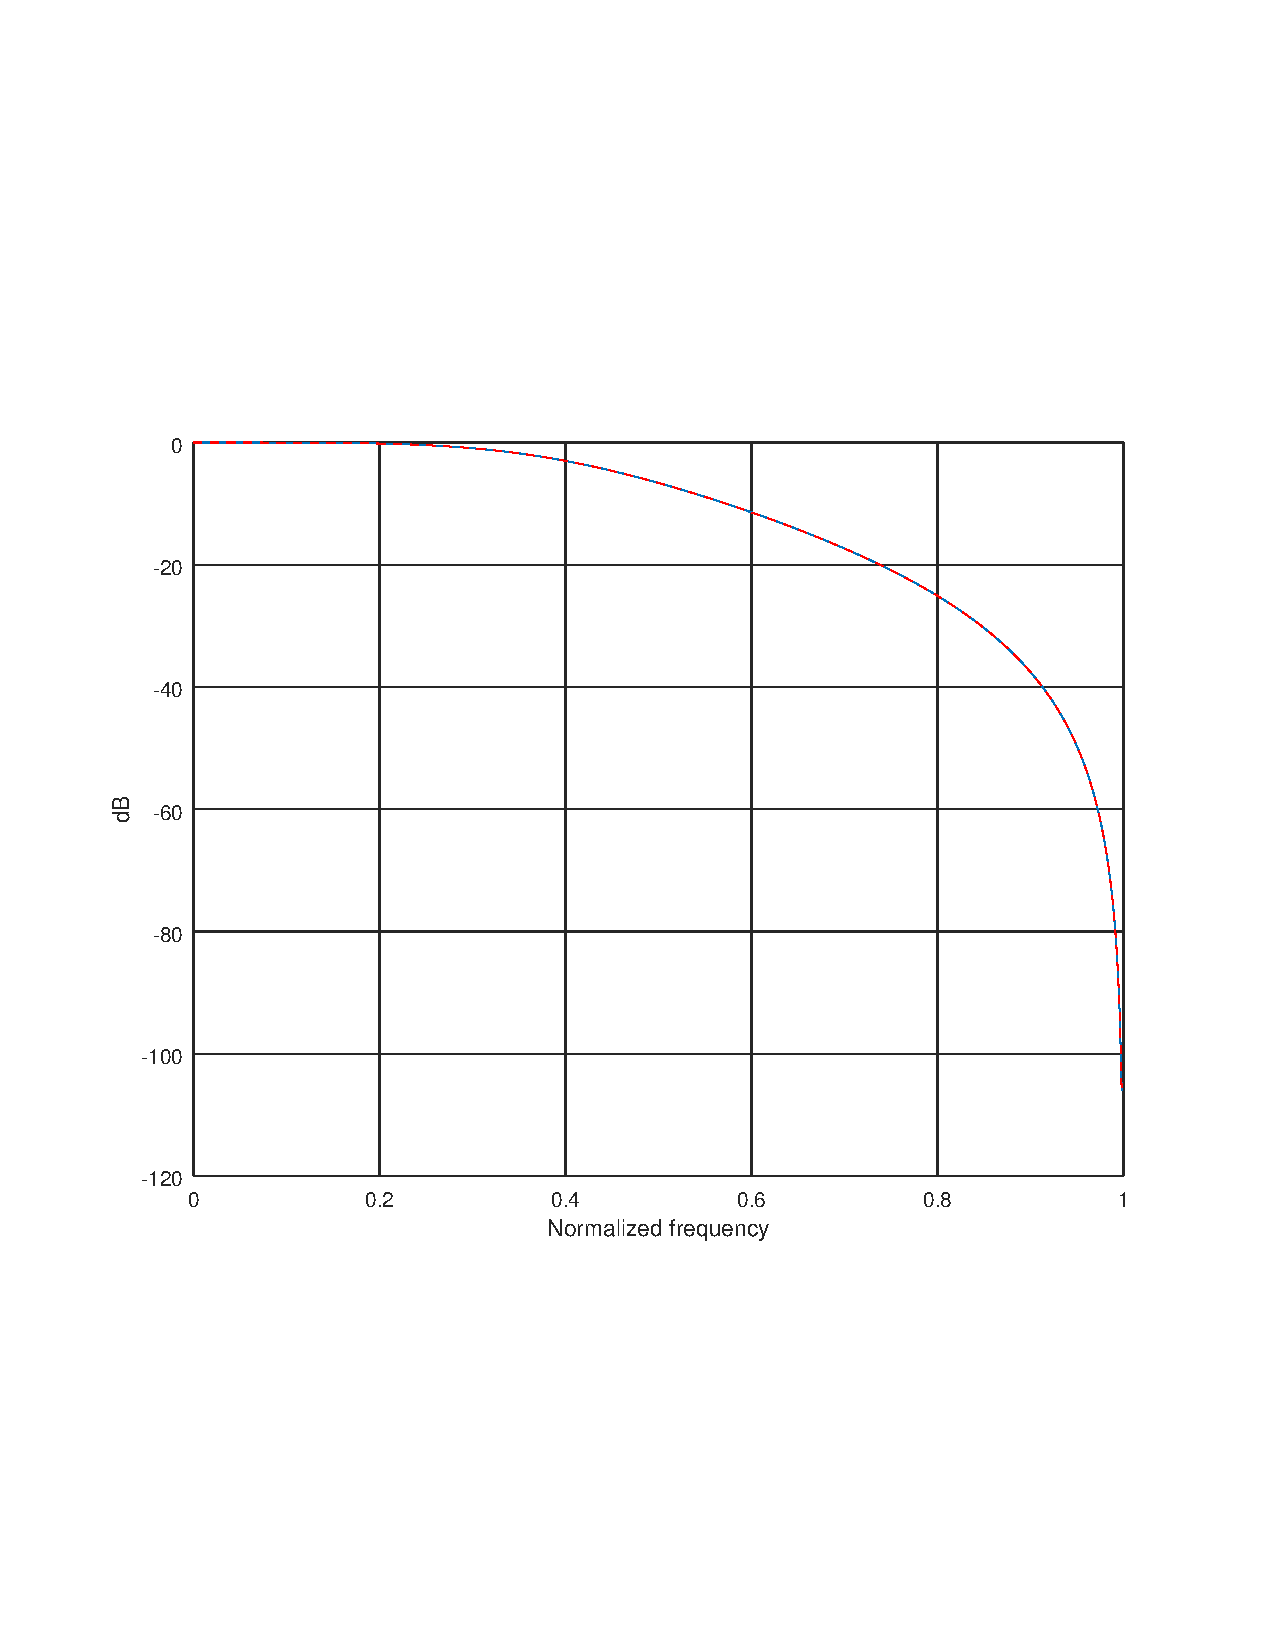
\includegraphics[width=.75\linewidth]{media/tf.pdf}
    \caption{Bode plot of the filter frequency response}
    \label{fig:tf}
\end{figure}
Figure~\ref{fig:tf} shows the transfer function of the filter computed from both the original coefficients and the quantized ones. The two curves cannot be told apart because the error is too small (\num{5.42e-7} in the worst case).

\begin{figure}[hbtp]
    \centering
    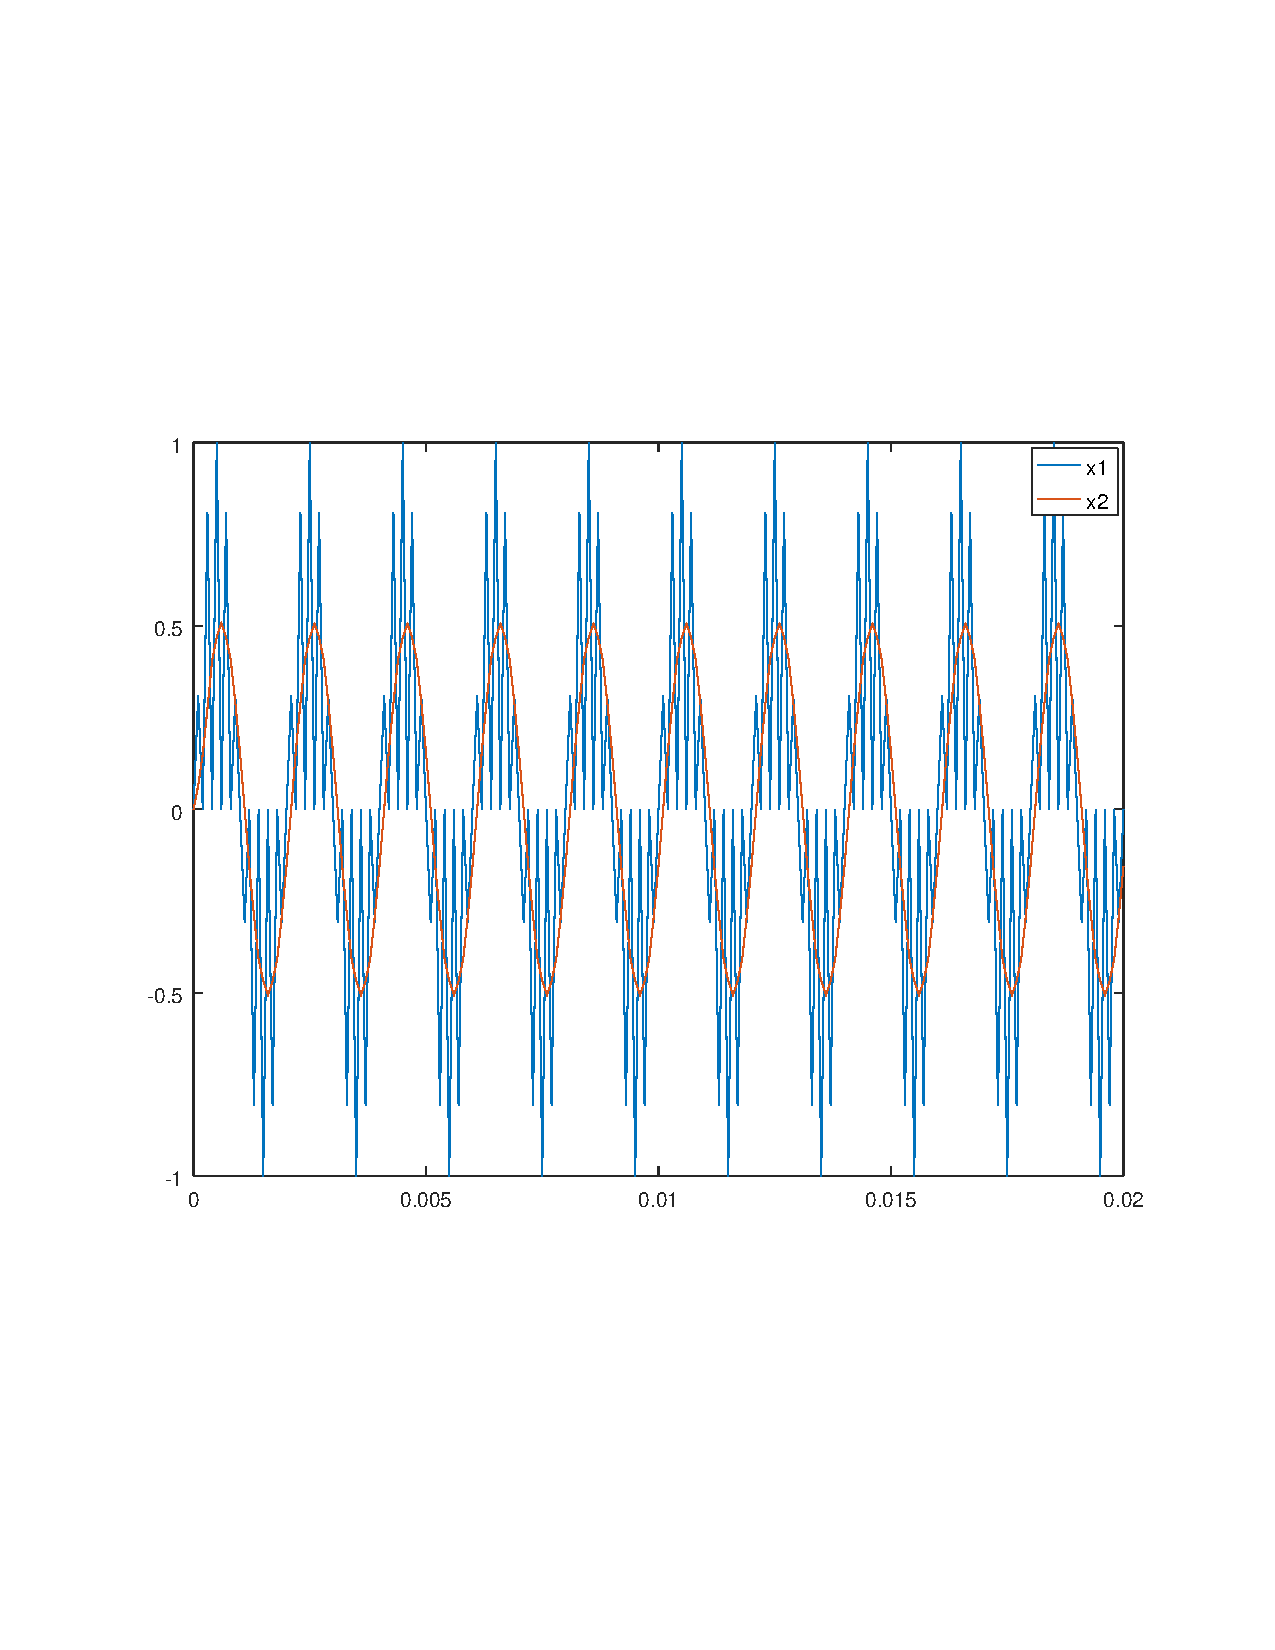
\includegraphics[width=.8\linewidth]{media/sine.pdf}
    \caption{Input and output waveforms}
    \label{fig:sine}
\end{figure}
Figure~\ref{fig:sine} on the other hand shows the time domain waveforms of an input signal $x_1(t)$, in blue, containing two frequency components one in band and one out of band, and the corresponding output $x_2(t)$, in red, where only the in-band component survives.

\section{Fixed-point C model}
The next step consists of writing a software model of the filter in C, which mirrors the behavior of the hardware architecture to be designed next. In this regard, the main difference between the MATLAB model and this one is that the former uses quantized coefficients but performs the internal computation using the maximum precision allowed by the machine, while the latter performs computation always resorting to the original fixed parallelism of data (12 bits here).

The development of this software model started with the example provided in the assignment, tailored to our specifications. A \href{https://github.com/mksoc/ISA-filter-design/blob/master/common/compare-outputs.py}{Python script} was developed and used to compare the results file of the two models. As expected, the comparison shows that the two models differ at most of one unity, that is the previously computed $\varepsilon_{max}$ (\ref{eq:emax}) in fractional form. Furthermore, results from the MATLAB model, when different, are always greater than the results from the C model, as the latter performs multiple truncations (rounding towards $-\infty$) in its computations. 

\section{Base architecture design}
The development of the first architecture began with the definition of the Data Flow Graph of the filter, shown in figure~\ref{fig:base_dfg}, from which the number of hardware resources needed can be derived (i.e. two delay elements, four adders and five multipliers).

\begin{figure}[hbtp]
    \centering
    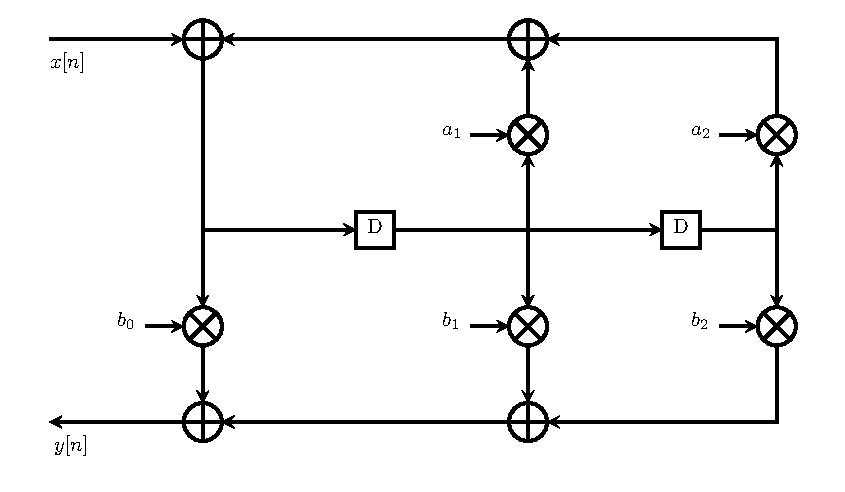
\includegraphics[width=.8\linewidth]{media/base_dfg.pdf}
    \caption{DFG of the filter}
    \label{fig:base_dfg}
\end{figure}

\subsection{Datapath}
From the generic DFG, a full datapath architecture was designed, shown in figure~\ref{fig:base_dp}. Compared to the simple DFG of figure~\ref{fig:base_dfg}, this datapath explicitly shows all signal names used throughout the design and their parallelism, along with additional interface registers required by the specifications. The following paragraphs detail the key points of the design. 

\begin{figure}[hbtp]
    \centering
    \makebox[\textwidth][c]{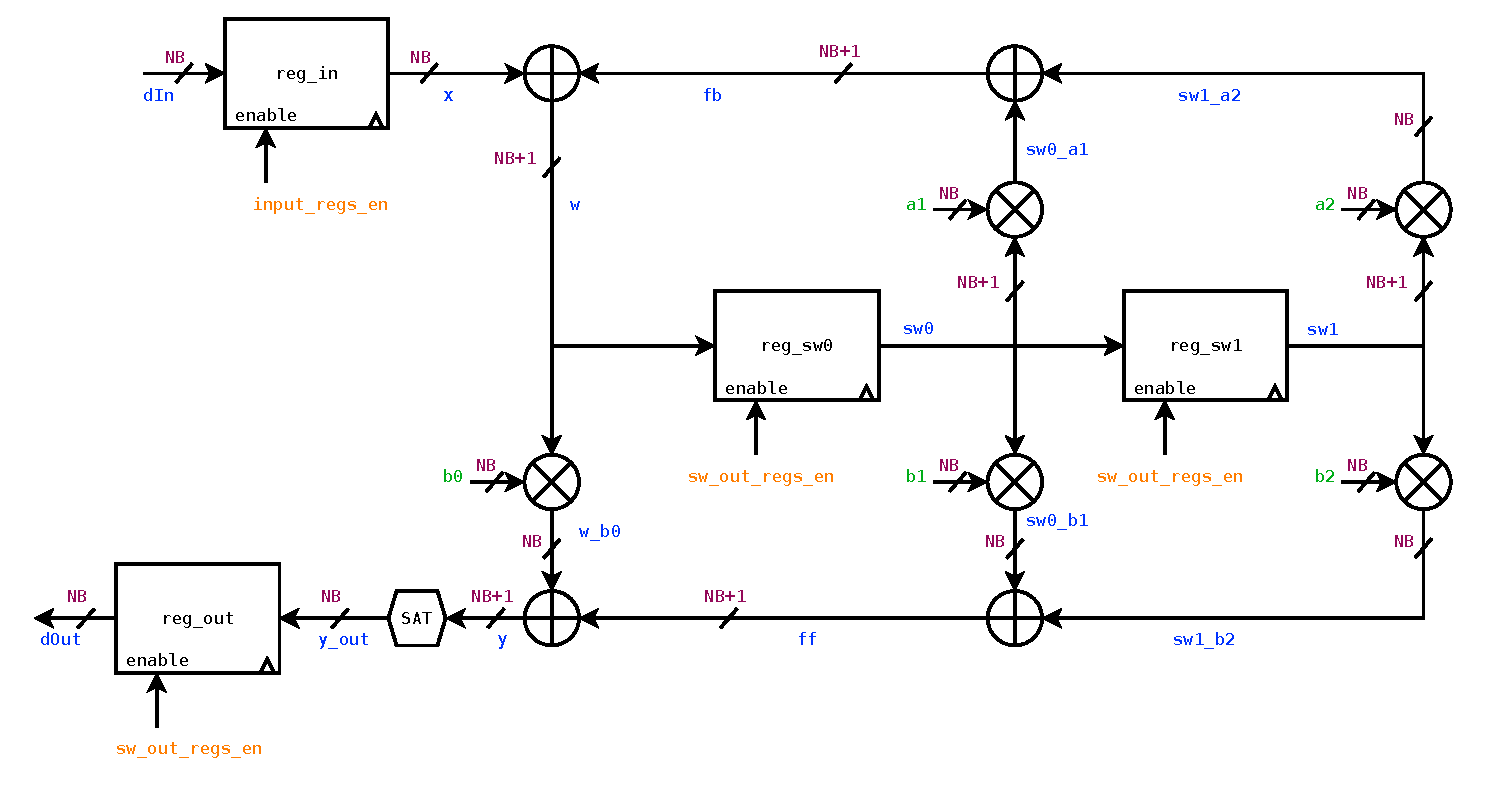
\includegraphics[width=1.25\linewidth]{media/base_dp.pdf}}
    \caption{Datapath}
    \label{fig:base_dp}
\end{figure}

\subsubsection{Color legend}
All datapath schemes used in this report follow the same color coding:
\begin{itemize}
    \item \textcolor{blue}{Blue} signals are data signals
    \item \textcolor{ForestGreen}{Green} signals are external coefficients
    \item \textcolor{Plum}{Purple} labels define the parallelism of the corresponding signal
    \item \textcolor{orange}{Orange} signals are control signals coming from the Control Unit
\end{itemize}

\subsubsection{Registers}
In addition to the two core delay elements of the filter DFG, the complete datapath includes also border registers for each piece of data coming in or out of the architecture, specifically the input and output sample stream and all filter coefficients. Input registers for the latter are not actually shown in figure~\ref{fig:base_dp} to avoid too much visual clutter, but assume that each coefficient in green is actually the output of a register.

Each register has implicit clock and asynchronous reset signals, as well as individual enable signals. No synchronous clear is provided as it is of no use for the purposes of this design.

\subsubsection{Arithmetic operators}
As per specifications, arithmetic operators at this stage of the design are described as behavioral operators in VHDL. While no rounding is requested after addition, each multiplication must truncate back to the original number of bits, a VHDL package was written, containing a function called \texttt{multiplyAndRound} which performs potential sign extension of the operands, behavioral multiplication and truncation. In the same package, some constants and custom data types to make the design parametric were defined as well.

Addition is more easily implemented as simply the behavioral operator `$+$', but the fact that addition can overflow and need an additional bit on the output posed the need for some considerations about internal parallelism. By performing an analysis on the specific values of filter coefficients and the range of data stream values, the conclusion was that the maximum internal parallelism that this specific architecture can need is: $$n_b+1 = \SI{13}{bit}$$

Contrary to the initial expectations however, the output value $y$ was found to need $(n_b+1)$ bits as well because of occasional overflow, while in the beginning it was expected to stay in the $n_b$ range. Overflow on the output would of course cause very large errors in the result because of wrapping. So it was decided to implement a saturation approach which limits the error instead, by taking the maximum or minimum value allowed on $n_b$ bits if the actual results is too large or too small to be represented correctly.

This decision led to the need of modifying the fixed-point C model as well, to provide the same results of the VHDL description to compare during simulation and testing.

\subsection{Control unit}
Given the simplicity of the design, it was initially thought that no explicit control unit would be needed. While it is actually possible to avoid it completely, some considerations about the ease of extending the design with subsequent transformations and pipelining (section~\ref{sec:improv}) as well as the preference for modularity and clarity led to the decision to implement a simple control unit, which FSM is shown in figure~\ref{fig:fsm}.

\begin{figure}[hbtp]
    \centering
    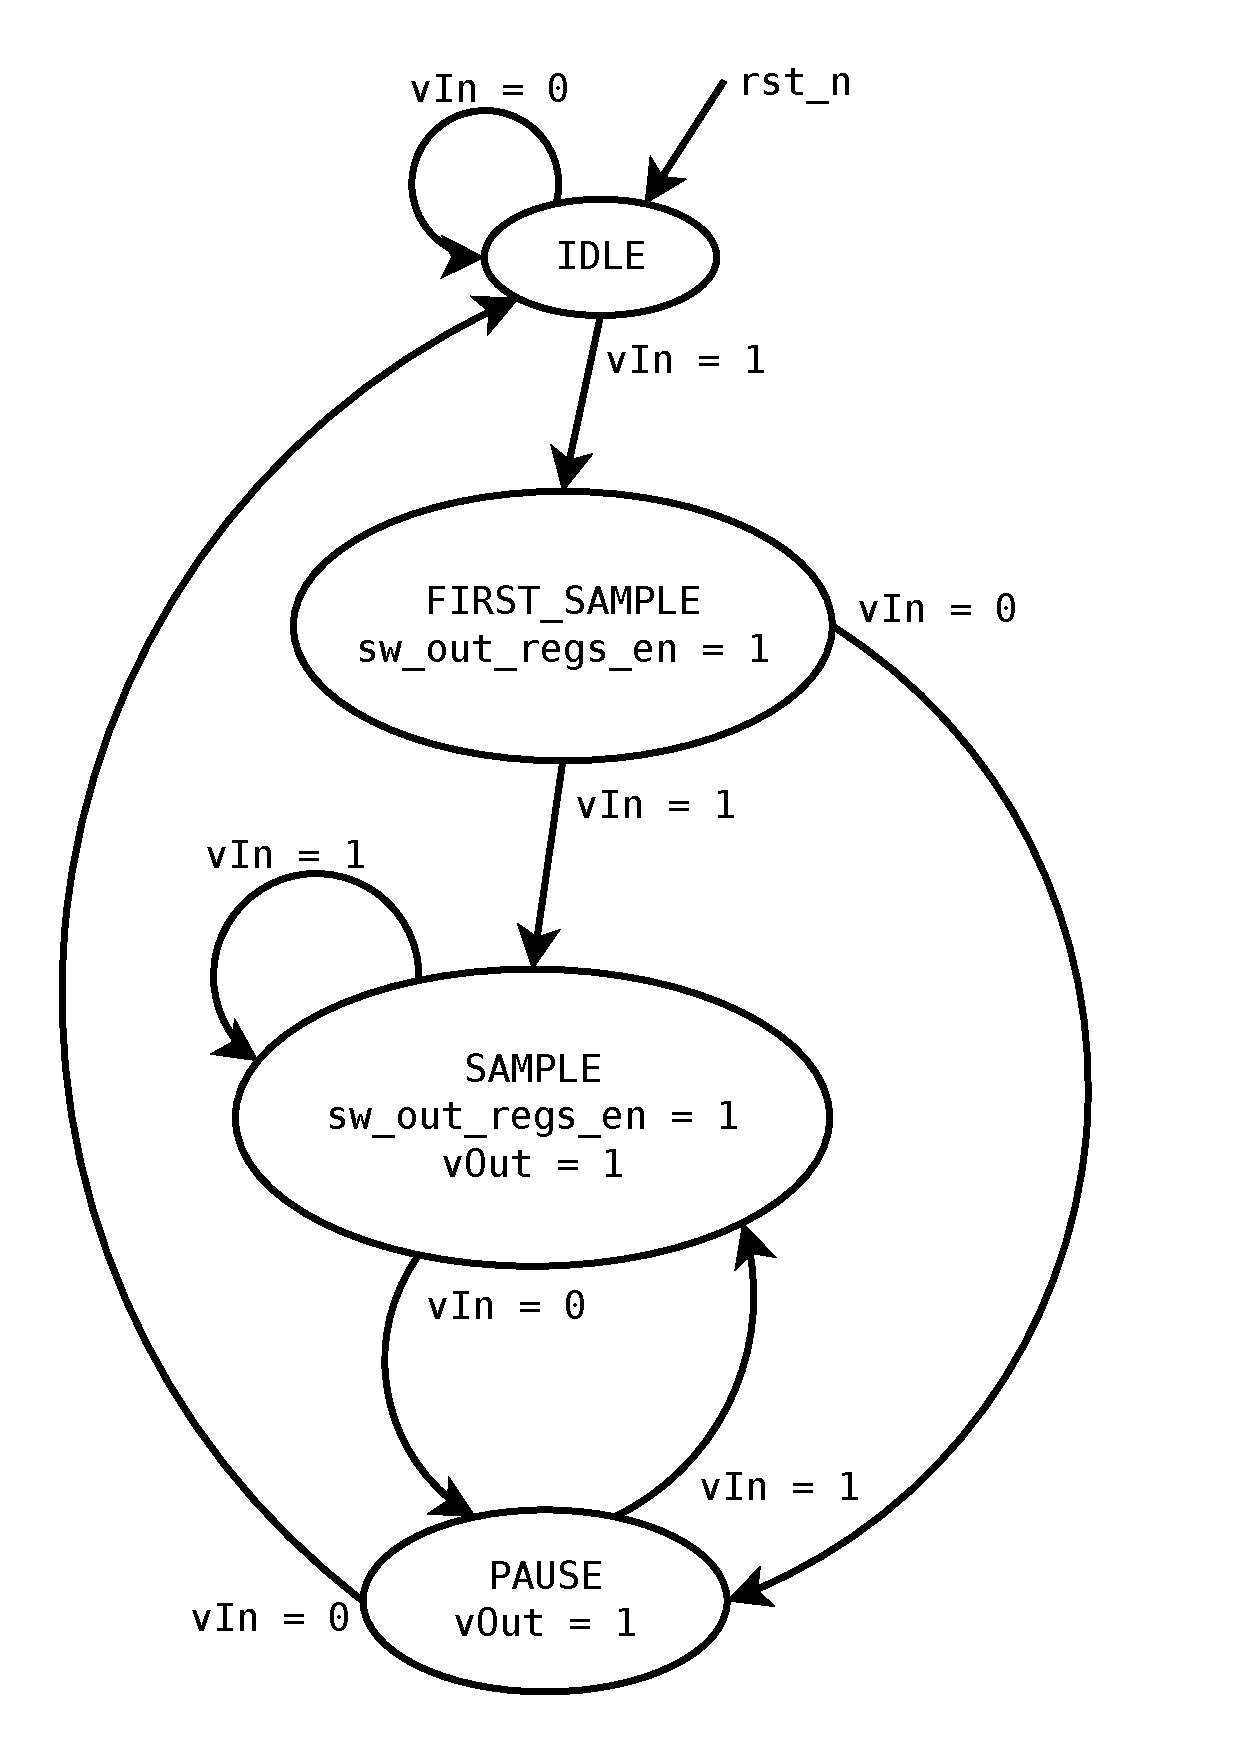
\includegraphics[width=.5\linewidth]{media/fsm.pdf}
    \caption{Filter control unit FSM}
    \label{fig:fsm}
\end{figure}

This control unit satisfies the specifications about the generation of the signal \texttt{vOut} to notify the presence of new data at the output and the need to take into account possible pauses during the input data stream. In practice, figure~\ref{fig:timing} shows the timing diagram that this FSM implements.

\begin{figure}[hbtp]
    \centering
    \makebox[\textwidth][c]{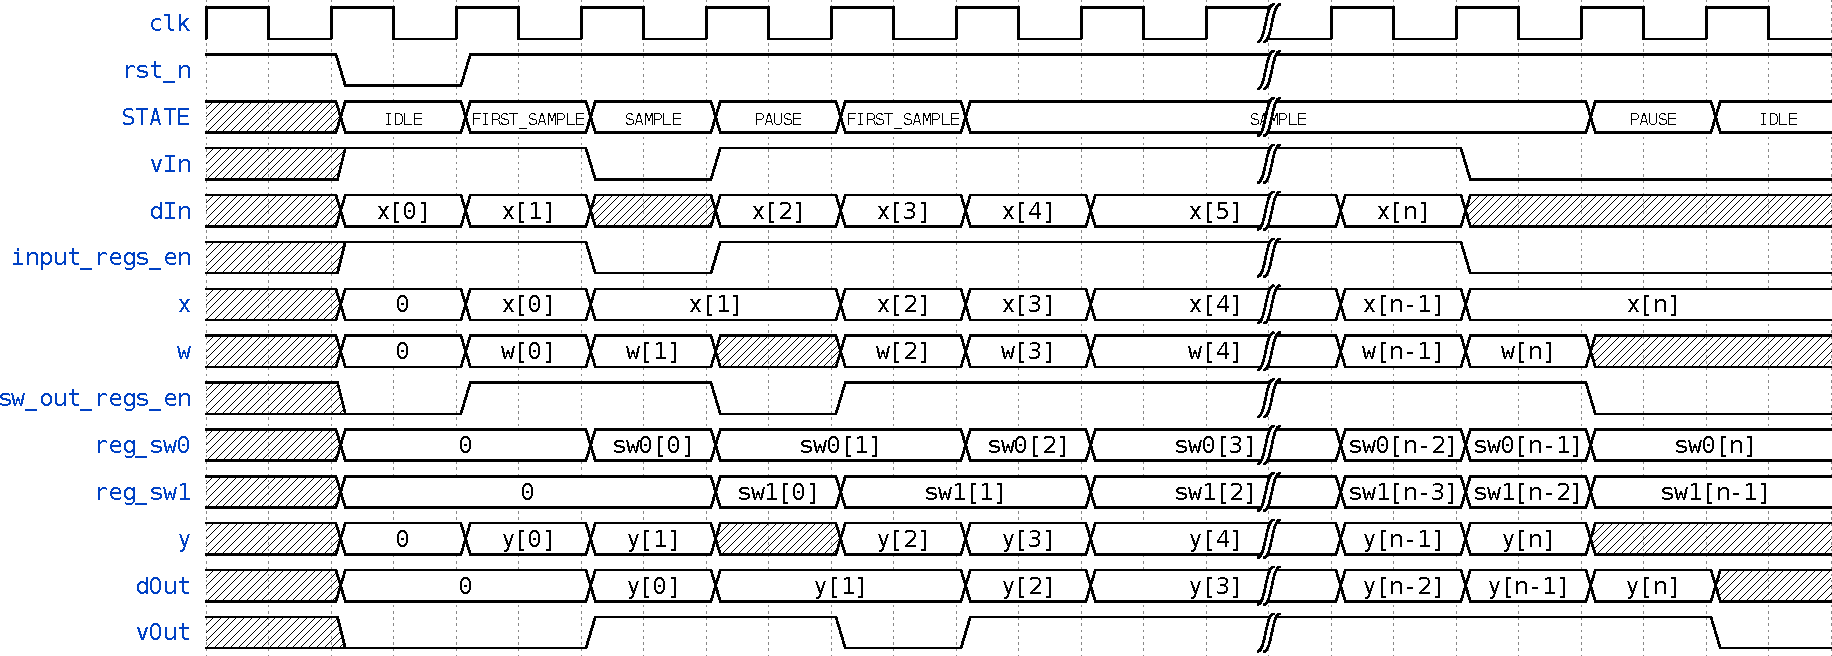
\includegraphics[width=1.25\linewidth]{media/timing.pdf}}
    \caption{Timing diagram}
    \label{fig:timing}
\end{figure}

\subsection{Simulation}
All simulations were performed using ModelSim both on our local machines and on the remote server, by means of a mixed-language testbench partly already provided in the course material. The procedure and tools described in the following sections apply to the simulation of all the RTL description as well as the netlists generated by other tools used for synthesis or place and route.

Each design or netlist has been simulated extensively multiple times using up to 100000 samples generated randomly or with special values, which would normally take around 20 minutes.

Regarding the simulation of the RTL description, no particular problems arose apart from the usual initial debugging and in the end the design worked as expected.

\subsubsection{Testbench}
The testbench is made up of several independent modules:
\begin{itemize}
    \item A \emph{clock generator} in charge of generating the initial reset signal and a periodic clock of specified period until an external \texttt{end\_sim} signal arrives to notify the end of the simulation. This is useful to automatically stop the simulation process when all input data has been processed instead of fixing a specific time span a priori.
    \item A \emph{data maker} which reads input data from a text file, converts it to a suitable format (\texttt{signed} in this case) and feeds it to the hardware description of the filter. It also allows to insert pauses in between samples to verify that such situation is handled correctly by the design. The number of pauses can be hard-coded or random, according to the value of a constant defined in the package.
    \item A \emph{data sink} to read output data stream from the hardware block and write it to another text file.
    \item A top module written in Verilog (instead of VHDL as the previous ones) that simply connects the instance of the filter and all other testbench modules together. The need to describe this block in Verilog arises from the fact that synthesis and place and route tools generate Verilog netlists and are more comfortable using Verilog files.
\end{itemize}

\subsubsection{Scripts}
In order to try to automate as much as possible the simulation process, a number of scripts were developed, which can be found in the GitHub repository or in the material provided:
\begin{itemize}
    \item \texttt{samples-generator.py} to generate a user-specified number of samples either random or special (meaning extremes and zero only).
    \item \texttt{auto-scp.sh} to automate the copy of source files and input samples on the server and results and netlists from the server.
    \item \texttt{compare-results.py} which compares the results of the simulation against the ones produced by the C model (figure~\ref{fig:yeee}).
    \item \texttt{auto-simulate.sh} which allows, by means of defining environmental variables, to choose whether to simulate locally or remotely and which design to simulate (RTL description, post-synthesis netlist or post-place and route netlist) and then performs several steps to automatically carry out the simulation, namely:
    \begin{itemize}
        \item Generates samples using \texttt{samples-generator.py}.
        \item Runs the C model on these samples.
        \item Connects to the server (if the user has chose to run the simulation remotely) and copies the samples file.
        \item Runs ModelSim CLI to perform the simulation.
        \item Retrieves output files and compare the results.
    \end{itemize}
    \item \texttt{sim-script.tcl} executed directly by ModelSim, which reads the environmental variables passed by \texttt{auto-simulate.sh} and issues the correct commands to the tool.
\end{itemize}

\begin{figure}[hbtp]
    \centering
    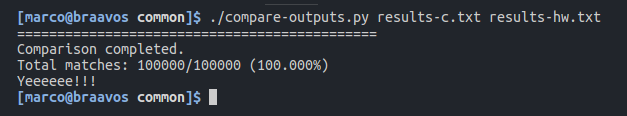
\includegraphics[width=.8\linewidth]{media/2018-12-20-143134_627x116_scrot.png}
    \caption{Successful comparison}
    \label{fig:yeee}
\end{figure}

\subsection{Synthesis}
The synthesis of the design has been carried out using Synopsys Design Compiler, following the instructions given in the specifications. All the commands issued to the tool were again put together inside a TCL script to ease the repetition of the process. 

At first try, the comparison between the synthesized design and the original RTL description resulted in outputs being completely different. After some trial and error, which included confrontation with colleagues and Professors, the issue came out to be the issuing of asynchronous reset signal in the first state of the control unit to all registers. The solution was to remove those outputs from such state and instead wire up the reset of the register directly to the external reset signal, which rendered the initial state of the control unit an empty idle state, as seen in the final FSM of figure~\ref{fig:fsm}.

After successfully completing the synthesis and testing the correctness of the results from the netlist, we extracted two figures of merit: the first at the maximum achievable frequency, that is shown in table~\ref{tab:base_post_syn_maxf}, and the second at a quarter of this frequency, shown in table~\ref{tab:base_post_syn}

\begin{table}[hbtp]
    \centering
    \begin{tabular}{|l|l|}
    \hline
    $f_{max}$     & $\SI{352.11}{MHz}$              \\ \hline
    Area          & $\SI{4705.51}{\micro\meter^2}$  \\ \hline
    Dynamic power & $\SI{86.13}{\micro\watt}$       \\ \hline
    Static power  & $\SI{16.53}{\micro\watt}$       \\ \hline
    \end{tabular}
    \caption{Figures of merit post-synthesis at $f_{max} = \SI{352.11}{MHz}$.}
    \label{tab:base_post_syn_maxf}
\end{table}

\begin{table}[hbtp]
    \centering
    \begin{tabular}{|l|l|}
    \hline
    $f$           & $\SI{88.0}{MHz}$                \\ \hline
    Area          & $\SI{3915.25}{\micro\meter^2}$  \\ \hline 
    Dynamic power & $\SI{84.41}{\micro\watt}$       \\ \hline
    Static power  & $\SI{966.11}{\nano\watt}$       \\ \hline
    \end{tabular}
    \caption{Figures of merit post-synthesis at $f_{max}/4 = \SI{88.0}{MHz}$.}
    \label{tab:base_post_syn}
\end{table}

These results show a reduction of $94\%$ on the leakage power, that has now almost no impact on the total power consumption of the chip. 

\subsection{Place \& route}
The place and route phase was carried out using Cadence Innovus and the instructions provided in the lab track. As always, a script was put together to collect all commands issued to the tool, even if it was more difficult in this case as the GUI was heavily used. 

All the place and route was done using a clock frequency equal to a quarter of the maximum one found during synthesis. At the end of the process, three layers of metal interconnections were used. The results are shown in table~\ref{tab:base_post_pnr}.

\begin{table}[hbtp]
    \centering
    \begin{tabular}{|l|l|}
    \hline
    $f$           & $\SI{88.0}{MHz}$                \\ \hline
    Area          & $\SI{3904.3}{\micro\meter^2}$   \\ \hline 
    Dynamic power & $\SI{1.381}{\milli\watt}$      \\ \hline 
    Static power  & $\SI{78.7}{\micro\watt}$        \\ \hline
    \end{tabular}
    \caption{Figures of merit post-place \& route. Both area and power were computed at $f_{max}/4 = \SI{88.0}{MHz}$ as per laboratory guidelines.}
    \label{tab:base_post_pnr}
\end{table}

\subsection{Remarks}
\label{sec:base_remarks}

By comparing tables~\ref{tab:base_post_syn} and~\ref{tab:base_post_pnr}, it is possible to see how the early, post-synthesis estimation of the chip area is quite consistent with the place and route results. However, the reported dynamic and static power are quite different. In fact, the dynamic power is about $16$ times higher, while the static power (leakage) is about $80$ times higher, even worse than the expected leakage power of the same chip working at $f_{max}$. The explanation can be found in the fact that the synthesis doesn't take into account interconnections and power rings. The introduced capacitance might be a reason for the dynamic power to be increased. On the other hand, the huge increase in leakage power is something we are not able to explain properly. Innovus reported high leakage in the combinational logic ($87\%$ of total static power). Maybe this is related to the the necessity of driving the metal interconnections. 

Comparing our results with those from other groups, we noticed that, in general, FIR filters brought to better results in terms of consistency between post-synthesis and post-place and route power reports. This might be explained by by considering that FIR filter are usually bigger (higher order), to obtain a frequency response as steep as the one from an IIR filter. For this reason, the introduced capacitance and logic required to drive the interconnections in a FIR filter might have a lower impact on the overall power performance of the chip with respect to an IIR filter, that contains fewer combinational and sequential nodes. 

\section{Look-ahead transform}\label{sec:improv}
The next step consists of improving the previous basic design by means of formal transformations and pipelining. Being the case in exam a IIR filter, the method implemented is the so-called \emph{look-ahead} transform, which consists of expanding the difference equation of the original filter (see~\ref{eq:diff}) by making explicit the term $y[n-1]$ as follows:
\begin{equation*}
    y[n-1] = b_0x[n-1] + b_1x[n-2] + b_2x[n-3] - a_1y[n-2] - a_2y[n-3]
\end{equation*}
Resulting in this final form of the difference equation:
\begin{equation}\label{eq:lookahead}
\begin{split}
    \rightarrow y[n] &= \!\begin{multlined}[t]
    \rightarrow   b_0x[n] + b_1x[n-1] + b_2x[n-2] - a_1\left(b_0x[n-1]+ b_1x\rightarrow n-2]+\right. \\
        \left.\rightarrow +\ b_2x[n-3] - a_1y[n-2] - a_2y[n-3]\right) - a_\rightarrow  [n-2]
    \end{multlined} \\
    &= \!\begin{multlined}[t]
        b_0x[n] + (\textcolor{ForestGreen}{b_1-a_1b_0})x[n-1] + (\textcolor{ForestGreen}{b_2-a_2b_1})x[n-2] + \\
        -\textcolor{ForestGreen}{a_1b_2x}[n-3] + (\textcolor{ForestGreen}{a_1^2-a_2})y[n-2] + (\textcolor{ForestGreen}{a_1a_2})y[n-3]
    \end{multlined} \\   
\end{split}
\end{equation}
The green highlights the fact that new coefficients different from the originals arise from the look-ahead transformation, which will necessitate adapting the parallelism and the hardware component to these new values.
Figure~\ref{fig:lookahead_dfg} shows the modified DFG that implements equation~\ref{eq:lookahead}.

\begin{figure}[hbtp]
    \centering
    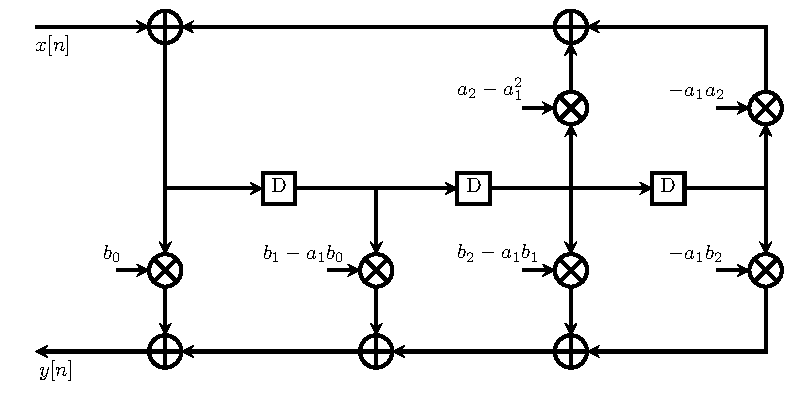
\includegraphics[width=.9\linewidth]{media/lookahead_dfg.pdf}
    \caption{Look-ahead transformed DFG}
    \label{fig:lookahead_dfg}
\end{figure}

\subsection{Loop bound analysis}
The justification for performing this modification on the original DFG lies in the analysis of the loop bound constrain and the critical path of the architecture. Figure~\ref{fig:base_dfg_lbcp} shows the loop bound (in blue) and the critical path (in green) on the original DFG, which values are respectively:
\begin{itemize}
    \item $T_\infty = 2T_a + T_m$
    \item $T_{cp} = 3T_a + 2T_m$
\end{itemize}
Being that $T_\infty < T_{cp}$, there is theoretically room for improvement even in the base architecture. In fact it is quite easy to see that pipelining could be applied in the FIR part of the DFG.

\begin{figure}[hbtp]
    \centering
    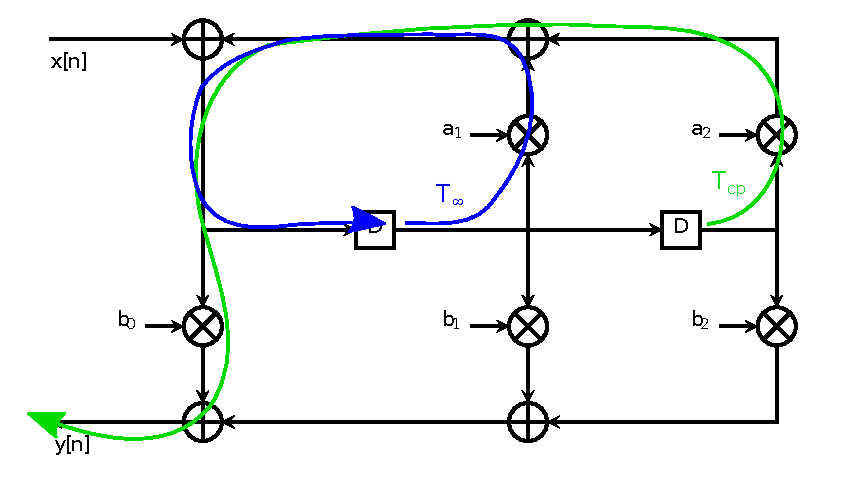
\includegraphics[width=.8\linewidth]{media/base_dfg_lbcp.pdf}
    \caption{Loop bound and critical path of the base DFG}
    \label{fig:base_dfg_lbcp}
\end{figure}

However, it makes more sense to apply improvements only on the modified DFG as the application of the look-ahead transform allows to halve the loop bound, as shown in figure~\ref{fig:lookahead_dfg_lbcp}, by introducing an additional delay element in the longest loop. 

\begin{figure}[hbtp]
    \centering
    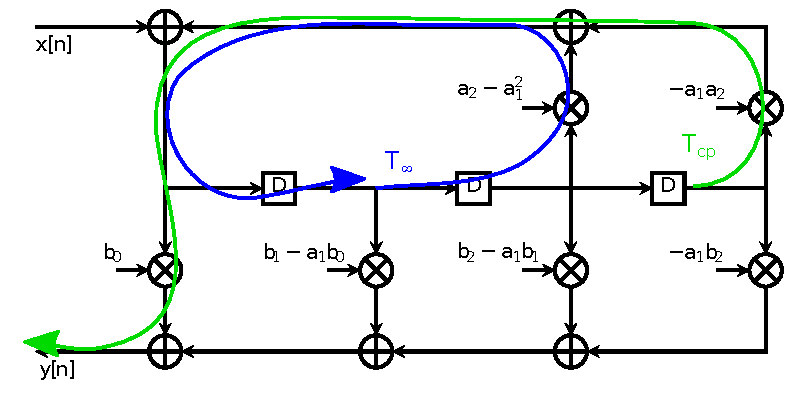
\includegraphics[width=.9\linewidth]{media/lookahead_dfg_lbcp.pdf}
    \caption{Loop bound and critical path of the look-ahead DFG}
    \label{fig:lookahead_dfg_lbcp}
\end{figure}

\subsection{Pipelining and retiming}
Figure~\ref{fig:lookahead_dfg_lbcp} shows also that the critical path remains exactly the same after the transformation, which means that the look-ahead transform on its own does not lead to any improvement at all, but simply enables speed-up to be achieved in other ways. 

In this particular case two different improvements can be performed on two different parts of the DFG:
\begin{itemize}
    \item \textbf{Pipelining}: in the feed-forward (or FIR) part of the filter two feed-forward cutsets can be identified and thus two levels of pipelining can be inserted. This reduces the critical path by excluding the last multiplier/adder couple from the total.
    \item \textbf{Retiming}: in the feedback (or IIR) part instead no feed-forward cutset can be identified (obviously), but retiming can be performed by splitting the second and third register in the delay line along the two forking branches and moving the copy in the IIR part after the two multipliers to exclude them from the critical path as well.
\end{itemize}
These transformations lead to the final DFG of figure~\ref{fig:pipelined_dfg}, where of course the loop bound is unchanged but the critical is reduced to the delay of a single multiplier $T_m$ \footnote{This is valid only if one multiplier is slower than three adders, but this is probably the case.}.

\begin{figure}[hbtp]
    \centering
    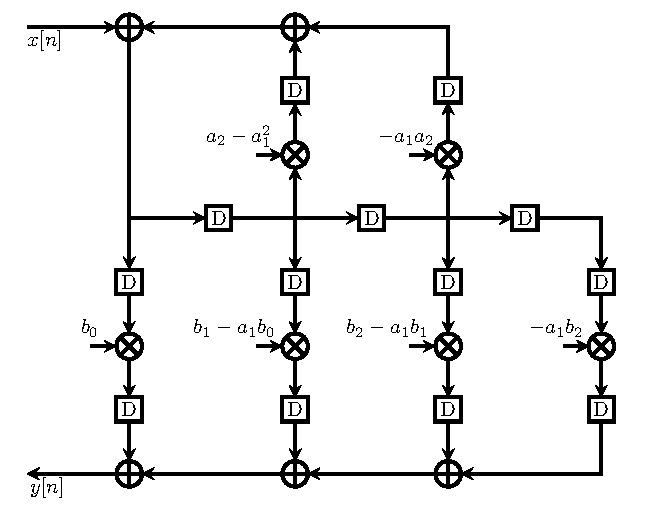
\includegraphics[width=.9\linewidth]{media/pipelined_lookahead_dfg.pdf}
    \caption{Final pipelined and retimed DFG}
    \label{fig:pipelined_dfg}
\end{figure}

Note that the loop bound is still smaller than the critical path, but no further improvement can be achieved without fine-grained pipelining inside the arithmetic operators, which is beyond the scope of this laboratory experience.

\subsection{Datapath}
\begin{figure}[hbtp]
    \centering
    \makebox[\textwidth][c]{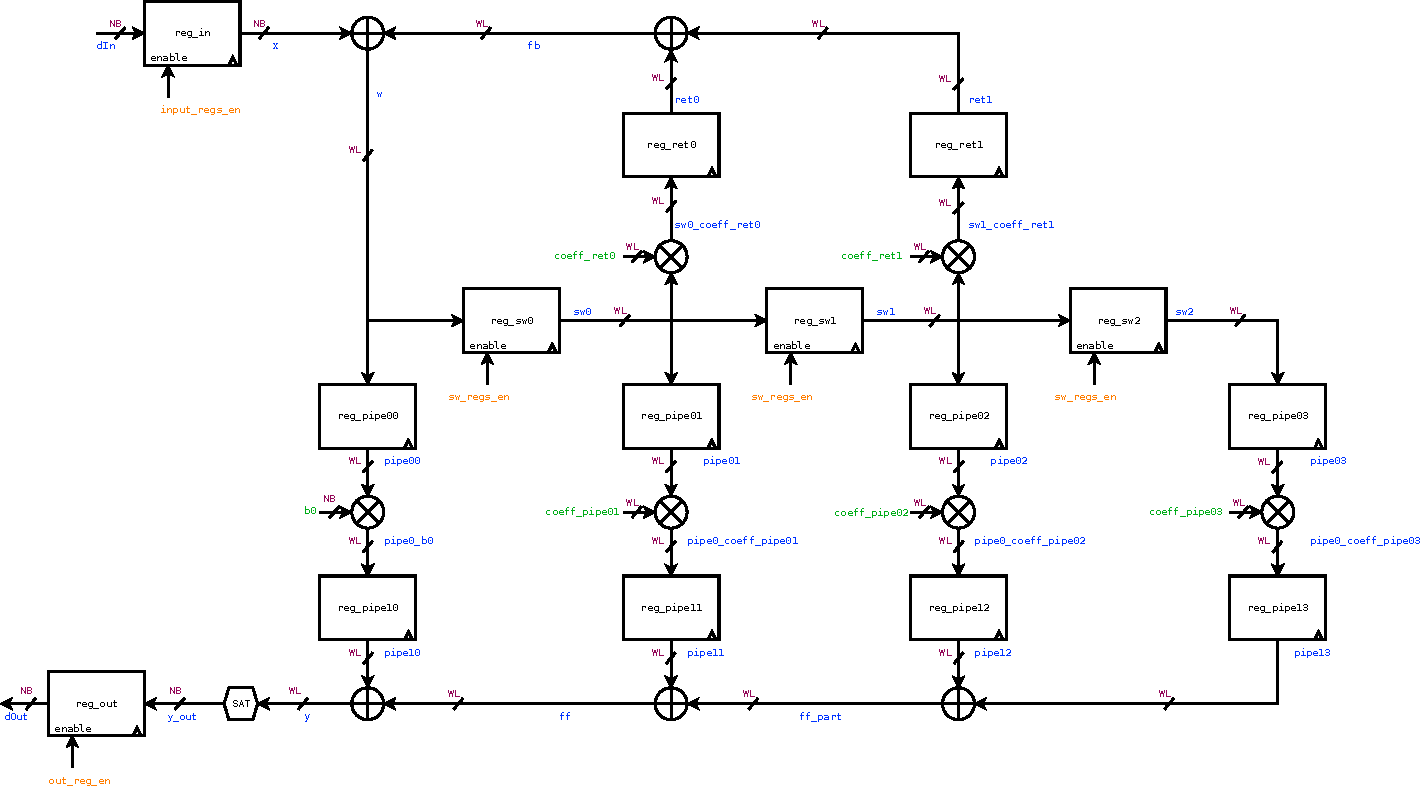
\includegraphics[width=1.3\linewidth]{media/pipelined_lookahead_dp.pdf}}
    \caption{Look-ahead datapath}
    \label{fig:pipelined_dp}
\end{figure}
Figure~\ref{fig:pipelined_dp} shows the detailed datapath of the new architecture. The color scheme used to illustrate signals is the same used before.

\subsubsection{Pipe registers}
Pipeline and retiming registers differ from the others as they do not have an \emph{enable} signal. This way they are ``free running'' and always sample after the initial reset. 
This choice was made to keep the design and the control as simple as before.

\subsubsection{Parallelism}
Having different coefficients expressed as sums and products of the original ones, the whole internal parallelism had to be recomputed. 

The maximum number of bits that these new coefficients require was found to be 23 bit ($Q1.22$ format, derived from the multiplication of two $Q1.11$ numbers which are less than $1$). Following the reasoning done for the original architecture, the multiplication function inside the VHDL package was modified to take care of the different parallelism and all the internal computations were chosen to be performed on 24 bits ($Q2.22$ format) to account for potential addition overflow. This number of bits was called \emph{word length} being the one used in all internal signals and is the one represented by the label \texttt{WL} in figure~\ref{fig:pipelined_dp}.

One last point that needed care was the alignment of external data streams (as well as the only coefficient that remained the same, $b_0$) which continue to be expressed in $Q1.11$ format, and thus require proper fixed point alignment and extension in both directions before getting summed with internal signals. 

As usual, the output is saturated in case of internal overflow.

\subsection{Control unit}
The great advantage of such pipelining process is that the control unit remains exactly the same as before, nothing at all needs to be modified.

The only change resides in the top level design, where a couple of signals coming from the control unit (namely, the output register enable and the data valid signal) have to be delayed of a number of clock cycles equal to the depth of the pipeline, to account for the additional latency of the output. 

This was very easy to implement, so that additionally the possibility to keep parametric the depth of the pipeline in the VHDL code was provided.

\subsection{Synthesis}
Table~\ref{tab:lookahead_post_syn_fmax} and table~\ref{tab:lookahead_post_syn} show the results obtained by the synthesis process on the look-ahead architecture. The procedure used for this as well as for the extensive simulation is exactly the same as before, so no additional detail have to be pointed out. 

% \textcolor{red}{PERÒ PORCO DIO NON HA SENSO UN CAZZO DI NIENTE. BUONANOTTE.} % Questa riga non verrà rimossa dalla sorgente per una semplice questione di "I know that feeling bro" dopo che ho smadonnato due giorni anche io sulle stesse cose... I feel you bro \m/

\begin{table}[hbtp]
    \centering
    \begin{tabular}{l|l|}
    \hline
    \multicolumn{1}{|l|}{$f_{max}$}     & $\SI{689.7}{MHz}$                 \\ \hline
    \multicolumn{1}{|l|}{Area}          & $\SI{18839.45}{\micro\meter^2}$   \\ \hline
    \multicolumn{1}{|l|}{Dynamic power} & $\SI{3.028}{\milli\watt}$         \\ \hline
    \multicolumn{1}{|l|}{Static power}  & $\SI{57.55}{\micro\watt}$         \\ \hline
    \end{tabular}
    \caption{Results of synthesis for the look-ahead architecture at $f_{max} = \SI{689.7}{MHz}$.}
    \label{tab:lookahead_post_syn_fmax}
\end{table}

\begin{table}[hbtp]
    \centering
    \begin{tabular}{l|l|}
    \hline
    \multicolumn{1}{|l|}{$f$}           & $\SI{172.41}{MHz}$                \\ \hline
    \multicolumn{1}{|l|}{Area}          & $\SI{15337.56}{\micro\meter^2}$   \\ \hline
    \multicolumn{1}{|l|}{Dynamic power} & $\SI{159.26}{\micro\watt}$        \\ \hline
    \multicolumn{1}{|l|}{Static power}  & $\SI{1.80}{\micro\watt}$          \\ \hline
    \end{tabular}
    \caption{Results of synthesis for the look-ahead architecture at $f = f_{max}/4 = \SI{172.41}{MHz}$.}
    \label{tab:lookahead_post_syn}
\end{table}

\subsubsection{Remarks}

Comparing these results, we can see how the dynamic power is reduced by $94\%$ when working at a quarter of the maximum frequency. Notice how this is consistent with the theoretical expectations. The dynamic power is a function of the clock frequency squared:
\begin{equation*}
    P_{dyn} \propto f^2 \Rightarrow P_{dyn} \left( f/4 \right) \approx P_{dyn} \left( f \right) = \frac{1}{16} P_{dyn} \left( f \right)
\end{equation*}

That is $1-1/16 = 94\%$ lower. 

Regarding the static leakage power, the reduction is consistent with the one obtained for the base architecture.

\subsection{Place \& route}
Again, the procedures followed to perform the place and rout and the related simulations on the lookahead implementation are the same as for the base architecture. Table~\ref{tab:lookahead_post_pnr} shows the obtained results. These were computed at $f = f_{max}/4 = \SI{172.41}{MHz}$. 

\begin{table}[hbtp]
    \centering
    \begin{tabular}{l|l|}
    \hline
    \multicolumn{1}{|l|}{$f$}           & $\SI{172.41}{MHz}$                \\ \hline
    \multicolumn{1}{|l|}{Area}          & $\SI{15231.4}{\micro\meter^2}$    \\ \hline
    \multicolumn{1}{|l|}{Dynamic power} & $\SI{4.511}{\milli\watt}$        \\ \hline
    \multicolumn{1}{|l|}{Static power}  & $\SI{323.6}{\micro\watt}$          \\ \hline
    \end{tabular}
    \caption{Results of place and route for the look-ahead architecture at $f = f_{max}/4 = \SI{172.41}{MHz}$.}
    \label{tab:lookahead_post_pnr}
\end{table}

\subsubsection{Remarks}
Comparing table~\ref{tab:lookahead_post_syn} and~\ref{tab:lookahead_post_pnr}, the conclusion are very similar to the ones already expressed for the base architecture. The post-synthesis area estimation was quite accurate, while the dynamic power has increased by $28\%$ after the place and route analysis. Also static power is, again, very different from the expected one from the synthesis process. However, the order of magnitude of the place and route results is the same as the ones from the first implementation. This supports the thesis expressed in section~\ref{sec:base_remarks}, that can be applied here as well. Of course, the datapath of the lookahead implementation is more complex than the original one, and this explains the increase in static and dynamic power. 

\end{document} 